\section{Introduction}
\label{sec:introduction}
Neural networks could be one of the most consequential artefacts humanity has built, yet we do not understand how they work or reliably control what they do. This is true despite humans designing the training procedure: we specify how models learn, but not what they learn. \emph{Interpretability} is the effort to understand what models learn and why they behave as they do, rather than only observing what they output. \emph{Mechanistic interpretability} (MI) is one approach within it. MI studies the \emph{internal mechanisms} (characterised in Section~\ref{subsec:circuits}) of the neural network in relation to its behaviour, which can yield both a richer understanding of the model and more reliable control over it.

Recent decades have seen an exponential improvement in AI capabilities~\citeem{touvron2023llamaopenefficientfoundation, openai2024gpt4technicalreport, gemmateam2024gemmaopenmodelsbased, yang2025qwen3technicalreport, deepseekai2025deepseekv3technicalreport, anthropic2025claude4}, but methods to understand and explain internal mechanisms have lagged behind. This has created an \emph{interpretability gap} between what models can do and what we know about how they do it. The gap is highly relevant for safety since standard behaviour-based safety measures, such as safety-oriented reinforcement learning from human feedback (RLHF)~(\citeemalp{bai2022training}; \citeestalp{dai2024safe}) and red-teaming~\citeest{perez2022redteaminglanguagemodels}, are not robust to sophisticated failure modes such as deceptive alignment~\citeem{hubinger2024sleeperagentstrainingdeceptive}. 


\begin{definitionbox}[The Interpretability Gap]
The \emph{interpretability gap} is the disparity between what models do (their capabilities and behaviours) and what we understand about how they do it (their internal mechanisms). As models scale, this gap risks widening: reasoning emerges that we cannot yet trace, deceptive behaviours may remain undetected, and safety guarantees built on incomplete understanding may fail unexpectedly.
\end{definitionbox}

\subsection{Brief History of Interpretability}

While early work did not establish interpretability as a distinct and clearly defined area of artificial intelligence, researchers sought to understand what neural networks learn long before the emergence of modern deep learning models such as transformers~\citeest{vaswani2017attention}. For example, \citetest{hinton1986distributed} discussed how representations of concepts can be distributed across multiple units, while \citetest{hinton1986learning} showed that networks can learn such distributed representations, with neurons encoding interpretable features of the concepts they represent. \citetest{elman1991distributed} further applied Principal Component Analysis (PCA; \citeestalp{pearson1901lines, hotelling1933analysis}) to the hidden states of a simple recurrent neural network~\citeest{elman1990finding} to analyse their trajectories as the network processed successive words in a sentence.

Even earlier, \citetest{minsky1969perceptrons} studied which functions or predicates particular neural architectures could and could not represent, and their results contributed to the temporary decline of neural-network research. 
While this earlier work was not driven by AI safety concerns, it was an early attempt to classify what neural networks can and cannot compute.

Modern efforts to understand the internals of neural networks began almost as soon as deep learning achieved practical success. \citetest{zeiler2014visualizing} developed visualisation techniques to inspect the convolutional filters that AlexNet~\citeest{NIPS2012_c399862d}, a convolutional neural network (CNN; \citeemalp{oshea2015introductionconvolutionalneuralnetworks}) architecture, had learned. Their study revealed that early layers detected edges, while deeper layers responded to increasingly complex patterns. \citetem{karpathy2015visualizing} and \citetest{li-etal-2016-visualizing} extended this approach to recurrent neural networks. By manually inspecting individual neurons, they discovered ones tracking various linguistic features, such as quotes, line lengths, brackets, negation, and syntactic structure. This showed empirically that an interpretable structure could emerge without explicit supervision.

These early works were largely manual: researchers examined individual neurons and reported qualitative findings. The field soon developed more systematic approaches. 

Probing classifiers~\citeest{belinkov-2022-probing} were popularised as a tool for studying neural representations through a series of works on linguistic structure and neural network analysis~\citeest{gupta-etal-2015-distributional, kohn-2015-whats, shi-etal-2016-string, adi2017finegrained, belinkov2017neural, conneau2018what, alain2017understanding}. These studies asked whether syntactic categories, semantic roles, or sentence length could be extracted from a layer's activations. \citetest{Dalvi_Durrani_Sajjad_Belinkov_Bau_Glass_2019} extended this approach to automatically identify individual neurons learning a concept by exploiting the weights of the probing classifier. %

This line of work flourished between 2016 and 2019, producing a rich catalogue of information that was present in model activations. 
It remains important for mechanistic interpretability research to consider carefully what conclusions can legitimately be drawn from the presence of information in a neural network. 

The introduction of transformers~\citeest{vaswani2017attention} and BERT~\citeest{devlin2019bert} intensified both the need and the opportunity for interpretability research. 
The attention mechanisms of these architectures allowed researchers to peer into the internal workings of models, spurring research on attention visualisation~(\citeestalp{vig2019multiscale}; \citeemalp{clark2019what, vig-belinkov-2019-analyzing}). In response, criticism and debates arose over whether attention was sufficient to explain model internals~\citeest{jain2019attention, wiegreffe2019attention}. Additionally, ``BERTology'' work~\citeest{rogers2020primer} shed light on transformer internals, and linguistic competence was tested via behavioural evaluations on curated datasets.


A series of feature visualisation studies~\citeem{olah2017feature} published through the \emph{Distill} publication~\citeem{distill_pub} argued that neural networks contain meaningful, human-interpretable features. \citetem{olah2020zoom} subsequently developed these ideas into the ``Circuits'' research programme, which framed neural networks as compositions of interpretable features connected by understandable algorithms. These early efforts laid the foundation of modern \emph{mechanistic interpretability}. 

These explorations later expanded to language models, with work on induction heads~\citeem{olsson2022incontextlearninginductionheads}, indirect object identification (IOI) circuits~\citeest{wang2022interpretabilitywildcircuitindirect}, and modular arithmetic and integer addition in toy models~(\citeestalp{nanda2023progressmeasuresgrokkingmechanistic, quirke2024understandingadditiontransformers}; \citeemalp{quirke2026understandingadditionsubtractiontransformers}). By mid-2024, sparse autoencoders (SAEs) enabled feature extraction at billion-parameter scale~(\citeestalp{cunningham2023sparse}; \citeemalp{templeton2024scaling}). We will discuss whether these methods provide complete mechanistic understanding in Section~\ref{sec:open_problems}.






\paragraph{Situating the Field.}
Early studies of neural network internals emerged in different research communities, including natural language processing (NLP)~\citeest{vig2019multiscale} and computer vision~\citeem{olah2017feature}. Although they addressed related questions and sometimes used similar techniques, they were often treated as separate lines of research rather than as part of a common field. The term \emph{mechanistic interpretability} (MI) became established as interest in neural networks' internal mechanisms grew and previously
scattered research communities increasingly converged under this term. From today's perspective, much earlier work~(\citeestalp{hinton1986learning, elman1991distributed, rnnfsa1992, OMLIN199641, zeiler2014visualizing}; \citeemalp{karpathy2015visualizing}) can also be considered part of MI's history, even though it predates the term and, in some cases, the broader field of AI interpretability. Today, the scope and standards of MI and AI interpretability are still evolving. For example, recent work argues that interpretability should meet higher scientific standards, such as producing claims that are both falsifiable and reproducible, and improving its use in model evaluations and downstream applications~(\citeemalp{lee2026rigorous, icml2025actionable}; \citeestalp{orgad2026position, biderman2026position}).

As a result, modern mechanistic studies are connected to a longer history of research on general AI interpretability~\citeest{Raukur2022TowardTA} and other domains. SAEs, for example, are built directly on decades of work in sparse coding and dictionary learning~(\citeestalp{olshausen1996emergence, lewicki2000learning, lee2006efficient}; \citeemalp{ng2011sparse}). Similarly, recent studies that discovered circuits in large language models~(\citeestalp{conmy2023automatedcircuitdiscoverymechanistic}; \citeemalp{ameisen2025circuit}) resonate with early work on extracting and formalising the internal mechanisms of recurrent neural networks as finite state automata~\citeest{rnnfsa1992, OMLIN199641}. Debates about attention-based explanations also echo earlier discussions of saliency maps~(\citeemalp{simonyan2014deepinsideconvolutionalnetworks, smilkov2017smoothgradremovingnoiseadding}; \citeestalp{ig, adebayo2020sanitycheckssaliencymaps}) and feature attribution~\citeest{lundberg2017unifiedapproachinterpretingmodel, ribeiro2016whyitrustyou, lrp}. %
This survey therefore connects contemporary \emph{mechanistic} methods to earlier research, tracing their foundations beyond the work that gained prominence after 2020.



\paragraph{Safety.}
Many studies in mechanistic interpretability are motivated by AI safety~(\citeestalp{burns2023discovering, detectvul}; \citeemalp{templeton2024scaling}). %
Researchers hope that understanding the internal workings of models will lead to better detection and control of critical model behaviours. But it is not clear if the current mechanistic approaches are suitable and sufficient for tackling crucial failure modes that are not well addressed by current behavioural or correlation-based methods. This concern motivates us to assess approaches not just by how well they provide understanding, but by the strength of their actionable impacts.

\paragraph{Curiosity and Discovery.}
Mechanistic interpretability is worth studying for reasons beyond safety applications. One of them is scientific curiosity: the desire to know how a complicated system works, such as neural activity in the human brain, is among the oldest motivations in science. Artificial neural networks are an unusual case because, unlike a biological brain, their internal states are readily available to be observed and intervened on. This direct access allows researchers to tackle challenging questions, such as what a model represents internally or whether a particular concept is encoded in it. 

Besides scientific curiosity, there are also prospects for genuine discovery. For example, a model trained on a complex task (e.g., chess or Go) may settle on solutions its developers did not or could not anticipate, and recovering the implemented mechanisms can surface knowledge that the model has found on its own, from implemented algorithms to implicit representations of the task~\citeest{conceptdef}. In this sense, interpretability is a way to learn from a model, not just to audit and control it.


Building on this history, recent interpretability research reflects two significant methodological shifts.


\paragraph{First, from manual to assisted analysis.} At current model sizes, manual inspection of features and circuits is impractical. Consequently, researchers have developed methods that automate parts of mechanistic interpretability research. In particular, sparse autoencoders are a key automation tool: without supervision they extract millions of features from model activations (\citeestalp{cunningham2023sparse}; \citeemalp{bricken2023monosemanticity,templeton2024scaling}). Other work has proposed pipelines to automatically identify candidate circuits (\citeestalp{conmy2023automatedcircuitdiscoverymechanistic}; \citeemalp{ameisen2025circuit}), use language models to generate natural-language feature explanations~(\citeestalp{paulo2025automatically}; \citeemalp{bills2023language}), and provide initial validation of mechanistic hypotheses. While human judgement remains essential, some automation has become necessary.

\paragraph{Second, divergence in research priorities.} Even within safety-driven mechanistic interpretability research, there are distinct approaches. Some prioritise immediate safety interventions, such as steering, monitoring, and concept erasure, without requiring complete mechanistic understanding~\citeem{nanda2025pragmatic}, while others advocate complete causal understanding of model computation, even where this requires substantial resources~\citeem{gao2025ambitious}. Another paradigm studies the learning trajectory rather than the behaviour of a fixed model checkpoint~(\citeestalp{sellam2021multiberts,biderman2023pythia, biderman2026position}; \citeemalp{simon2026there}). Separate threads emphasise automating interpretability workflows to enable domain experts to query and correct model behaviour~\citeem{barez2025automated}, studying learning dynamics to anticipate emergent capabilities before deployment~\citeem{hoogland2023towards}, exploring whether models themselves can serve as explainers of their own internals~\citeem{li2025traininglanguagemodelsexplain}, or intervening on training processes to control model behaviour~(\citeestalp{biderman2023pythia}; \citeemalp{lee2026steps}).

The divergence of these research directions reflects the complexity of the problem and the uncertainty surrounding it, including open questions about how to define successful outputs of interpretability research~\citeest{lotfi2026position}. Thus, this survey does not argue for a single approach; rather, it organises recent progress around shared technical foundations (Section~\ref{sec:foundations} onwards) and discusses trade-offs between different goals (Section~\ref{sec:orientations}). We aim to clarify how these directions differ in their assumptions, failure modes, and capabilities, providing researchers with a principled basis for selecting and combining methods according to their own scientific and practical objectives.

\paragraph{Useful Surveys That We Build On.}
Several surveys cover overlapping territory. \citetest{bereska2024mechanisticinterpretabilityaisafety} and \citetest{zhang2026locatesteerimprovepractical} surveyed mechanistic interpretability methods with a focus on safety applications. \citetest{belinkov-glass-2019-analysis} provided a broad primer on the interpretability of neural language models. \citetest{llmexplainsurvey} surveyed interpretability for large language models. 
\citetem{rai2024practical} provided a task-centric and beginner-friendly taxonomy and review of mechanistic interpretability for transformer-based language models, while \citetem{ferrando2024primer} offered a technical primer on interpreting the inner workings and known mechanisms of transformer-based language models. More specifically, \citetest{sajjad-etal-2022-neuron} surveyed neuron-level interpretation, covering methods to discover, interpret, and control individual neurons. At a similar granularity, \citetest{shu-etal-2025-survey} surveyed SAEs, covering different SAE architectures, feature explanation methods, evaluation, and applications.

Our survey differs from previous surveys in framing, scope, and emphasis. Specifically, we examine closely what interpretability can actually contribute to AI safety. The close examination is motivated by the fact that, although many prior studies in the interpretability community assume that mechanistic understanding directly implies safer systems, the assumption is in fact largely untested. Therefore, this survey considers not only what a method reveals about a model's internal computation, but also what it allows us to do in practice. We particularly discuss whether it supports safety-relevant tasks such as detecting deceptive behaviours or identifying dangerous capabilities, and whether those tasks can be achieved just as well without interpretability methods or insights.

We cover popular methods and techniques up to mid-2026, including but not limited to recent work on large-scale feature extraction and analysis, circuit discovery, activation verbalisers, and model architectures designed with interpretability in mind. Rather than presenting these methods as a catalogue, we organise them around the methodological ideas they share and explain new methods in relation to the problems or limitations that motivated them.

We also place modern mechanistic methods in their broader historical context. Many of their underlying ideas actually predate transformers~\citeest{hinton1986learning, elman1991distributed}, and several techniques now central to the field have clear antecedents in earlier work, such as early development of sparse coding~\citeest{olshausen1996emergence} for today's sparse autoencoders. Making these connections explicit helps distinguish new methodological developments from adaptations of older ideas to new settings and shows where current debates revisit discussions that have appeared before.

We further make the terminology and claims about mechanistic interpretability more precise. This is necessary because some fundamental notions such as ``concept'', ``feature'', and ``mechanistic interpretability'' are not used clearly and consistently across the literature~\citeem{saphra2024mechanistic}. The consequence is that works described as mechanistic interpretability can support different kinds of conclusions; for example, showing that a specific intervention can change the target behaviour is a much weaker claim than showing that the behaviour's internal mechanism is precisely identified. To tackle this issue, for each introduced method, we discuss the assumptions about model internals it requires, the mechanistic claims it supports, and the strength of the claims. By doing this, we can separate disagreements about their mechanistic claims from disagreements about terminology, objectively comparing these methods even when their original papers use different terms.


Additionally, we systematically discuss the evaluation practices of interpretability methods, which are often validated through intuitive plausibility rather than rigorous testing. We cover existing evaluation frameworks and metrics, identify gaps, and argue that the evaluation methodology and safety benchmarks are the field's most pressing open problems.

\subsection{Survey Scope}
\label{sec:scope}




Our survey's main focus is on mechanistic interpretability for transformers~\citeest{vaswani2017attention}, which aims to explain how transformers convert inputs into outputs by analysing internal representations and mechanisms. This \textit{mechanistic} analysis involves direct manipulation of model internals to establish causal claims about computation, and must meet two criteria:

\begin{enumerate}
    \item \textbf{Engagement with model internals:} Targeting intermediate representations, individual components (neurons, features, attention heads, and more), or any other learned parameters (such as normalisation, embedding, and unembedding). This is not limited to just input--output relationships.
    \item \textbf{Causal claims:} Analyses that involve interventions (such as ablation, patching, and steering) and establish cause-to-effect relationships, rather than just correlational analysis.
\end{enumerate}

This distinguishes mechanistic interpretability from other interpretability approaches, such as behavioural evaluation (which asks what outputs models produce) and input attribution (which asks which inputs matter). However, it should be noted that interpretability methods that are not themselves mechanistic can \textit{facilitate} mechanistic analysis. For instance, although vanilla probes can only identify what information is decodable from the activations, they can become mechanistic when the identified directions are tested and used to intervene on models. Input attribution methods help locate salient input features (e.g., pixels), and follow-up processes, such as ablating them, can test causal claims about their roles. A key distinction is between methods that only provide \textit{descriptions} (correlational) and methods that enable \textit{interventions} (causal). Because descriptive methods often provide the targets for intervention, we cover in depth methods that analyse internal computation and let us discuss them within a shared causal vocabulary; we treat more briefly methods that are either behavioural or, while mechanistic, need separate theoretical and conceptual foundations.

We cover the following in depth:
\begin{itemize}
    \item \textbf{Foundations and core hypotheses:} Foundational concepts for mechanistic interpretability, including behavioural versus mechanistic understanding, polysemanticity, features, transformer computation, and circuits (Section~\ref{sec:foundations}), together with core hypotheses that motivate and constrain later mechanistic methods, including linear representations, superposition, privileged access, and the universality and Platonic representation hypothesis (Section~\ref{sec:hypotheses}).
    \item \textbf{Feature extraction and representation analysis:} Sparse autoencoders and related feature-extraction methods, multi-layer feature analysis, probing classifiers, intermediate-representation decoding, model diffing, knowledge localisation, and representation engineering (Sections~\ref{sec:sae}, \ref{sec:intermediate-computation}, and~\ref{sec:representation}).





    \item \textbf{Circuit analysis and related causal methods:} Circuit discovery, ablation, activation patching, causal verification, and other related interventions for identifying and testing mechanisms (Section~\ref{sec:circuit}).

    \item \textbf{Learning dynamics:} Feature and mechanism formation, forecasting model behaviour across training, longitudinal analysis of model training, phase transitions and emergence, and interventions on the training process (Section~\ref{sec:training}).

    \item \textbf{Training data attribution:} Gradient-based influence functions, verbatim and corpus-based attribution, and other methods for attributing model behaviour to training examples (Section~\ref{sec:influence-functions}).

    \item \textbf{Evaluation:} Frameworks for assessing mechanistic interpretability claims, such as testing their validity, faithfulness, causal relevance, and robustness (Section~\ref{sec:evaluation-framework}).

    \item \textbf{Research orientations:} The goals, assumptions, and trade-offs of six major research orientations in contemporary AI interpretability (Section~\ref{sec:orientations}).

    \item \textbf{Safety applications:} The use of mechanistic understanding and approaches for safety applications, including concept erasure, knowledge editing, representation steering, mechanistic monitoring, and automated interpretability agents, together with their risks and failure modes (Section~\ref{sec:safety_applications}).

    \item \textbf{Open problems:} Outstanding conceptual and technical challenges in mechanistic interpretability, including necessity, evaluation, scalability, generalisability, adversarial robustness, alignment, ontology, proxy fidelity, and transferability beyond transformers (Section~\ref{sec:open_problems}).
\end{itemize}

Notably, training data attribution (TDA; Section~\ref{sec:influence-functions}) does not meet the two criteria and is generally not considered a tool for mechanistic analysis. 
We note that many TDA methods operate via gradients or verbatim search, instead of intermediate representations. These approaches credit the behaviour entirely to the training data, completely ignoring internal computations. But we nevertheless include TDA approaches here as interpretability workflows increasingly chain the two techniques, in which mechanistic analysis generates hypotheses or clues about a behaviour's origin, while data attribution or corpus search verifies these claims~\citeem{nla}. 
Parameter-response-based TDA methods (e.g., influence functions~\citeest{koh2020understandingblackboxpredictionsinfluence}) were also introduced as a top-down complement to mechanistic analysis, with the stated goal of connecting the influence of data to responsible model components~\citeem{grosse2023studyinglargelanguagemodel, habibi2026symbolicmechanisticdataattribution}, making TDA a tool for mechanistic ends. 

We cover only post-hoc TDA methods that analyse a trained model. Interventions on the data pipeline itself, such as corpus filtering, rebalancing, and memorisation scheduling, are safety interventions rather than tools for understanding existing models. They are out of this survey's scope.

We discuss but do not cover in depth:
\begin{itemize}
    \item \textbf{Behavioural evaluation:} Red-teaming, benchmarks, and capability evaluations~(\citeemalp{ganguli2022redteaminglanguagemodels}; \citeestalp{perez2022redteaminglanguagemodels}). These studies assess what models do without explaining how. Section~\ref{sec:interpretability-landscape} discusses when behavioural methods may or may not suffice.
    \item \textbf{Input attribution:} SHAP~\citeest{lundberg2017unifiedapproachinterpretingmodel}, LIME~\citeest{ribeiro2016whyitrustyou}, integrated gradients~\citeest{ig}, and saliency maps~\citeem{simonyan2014deepinsideconvolutionalnetworks}. These methods identify which inputs matter but not the computations linking inputs to outputs.
    \item \textbf{Concept-based models:} 
    This class of models, especially concept bottleneck models (CBMs)~\citeest{koh2020conceptbottleneckmodels}, constrains models to route computation through human-specified concepts. These approaches involve direct manipulation of the computation and could be considered mechanistic; we discuss their relationship to other methods in Section~\ref{subsec:cbm}.
    \item \textbf{Causal abstraction:} Work on aligning model computations to high-level causal graphs~\citeest{geiger2021causalabstractionsneuralnetworks, pmlr-v162-geiger22a, das, JMLR:v26:23-0058, wu-etal-2022-causal}. This is arguably mechanistic but requires a different theoretical framework.%
\end{itemize}

See Figure~\ref{fig:simplified-taxonomy} for the complete taxonomy of topics and some representative papers covered in this work, and Figure~\ref{fig:overview} for an overview of the survey's structure.

















    
    
    
    
    
    
    
    
    

\begin{figure}[tb]
  \centering
  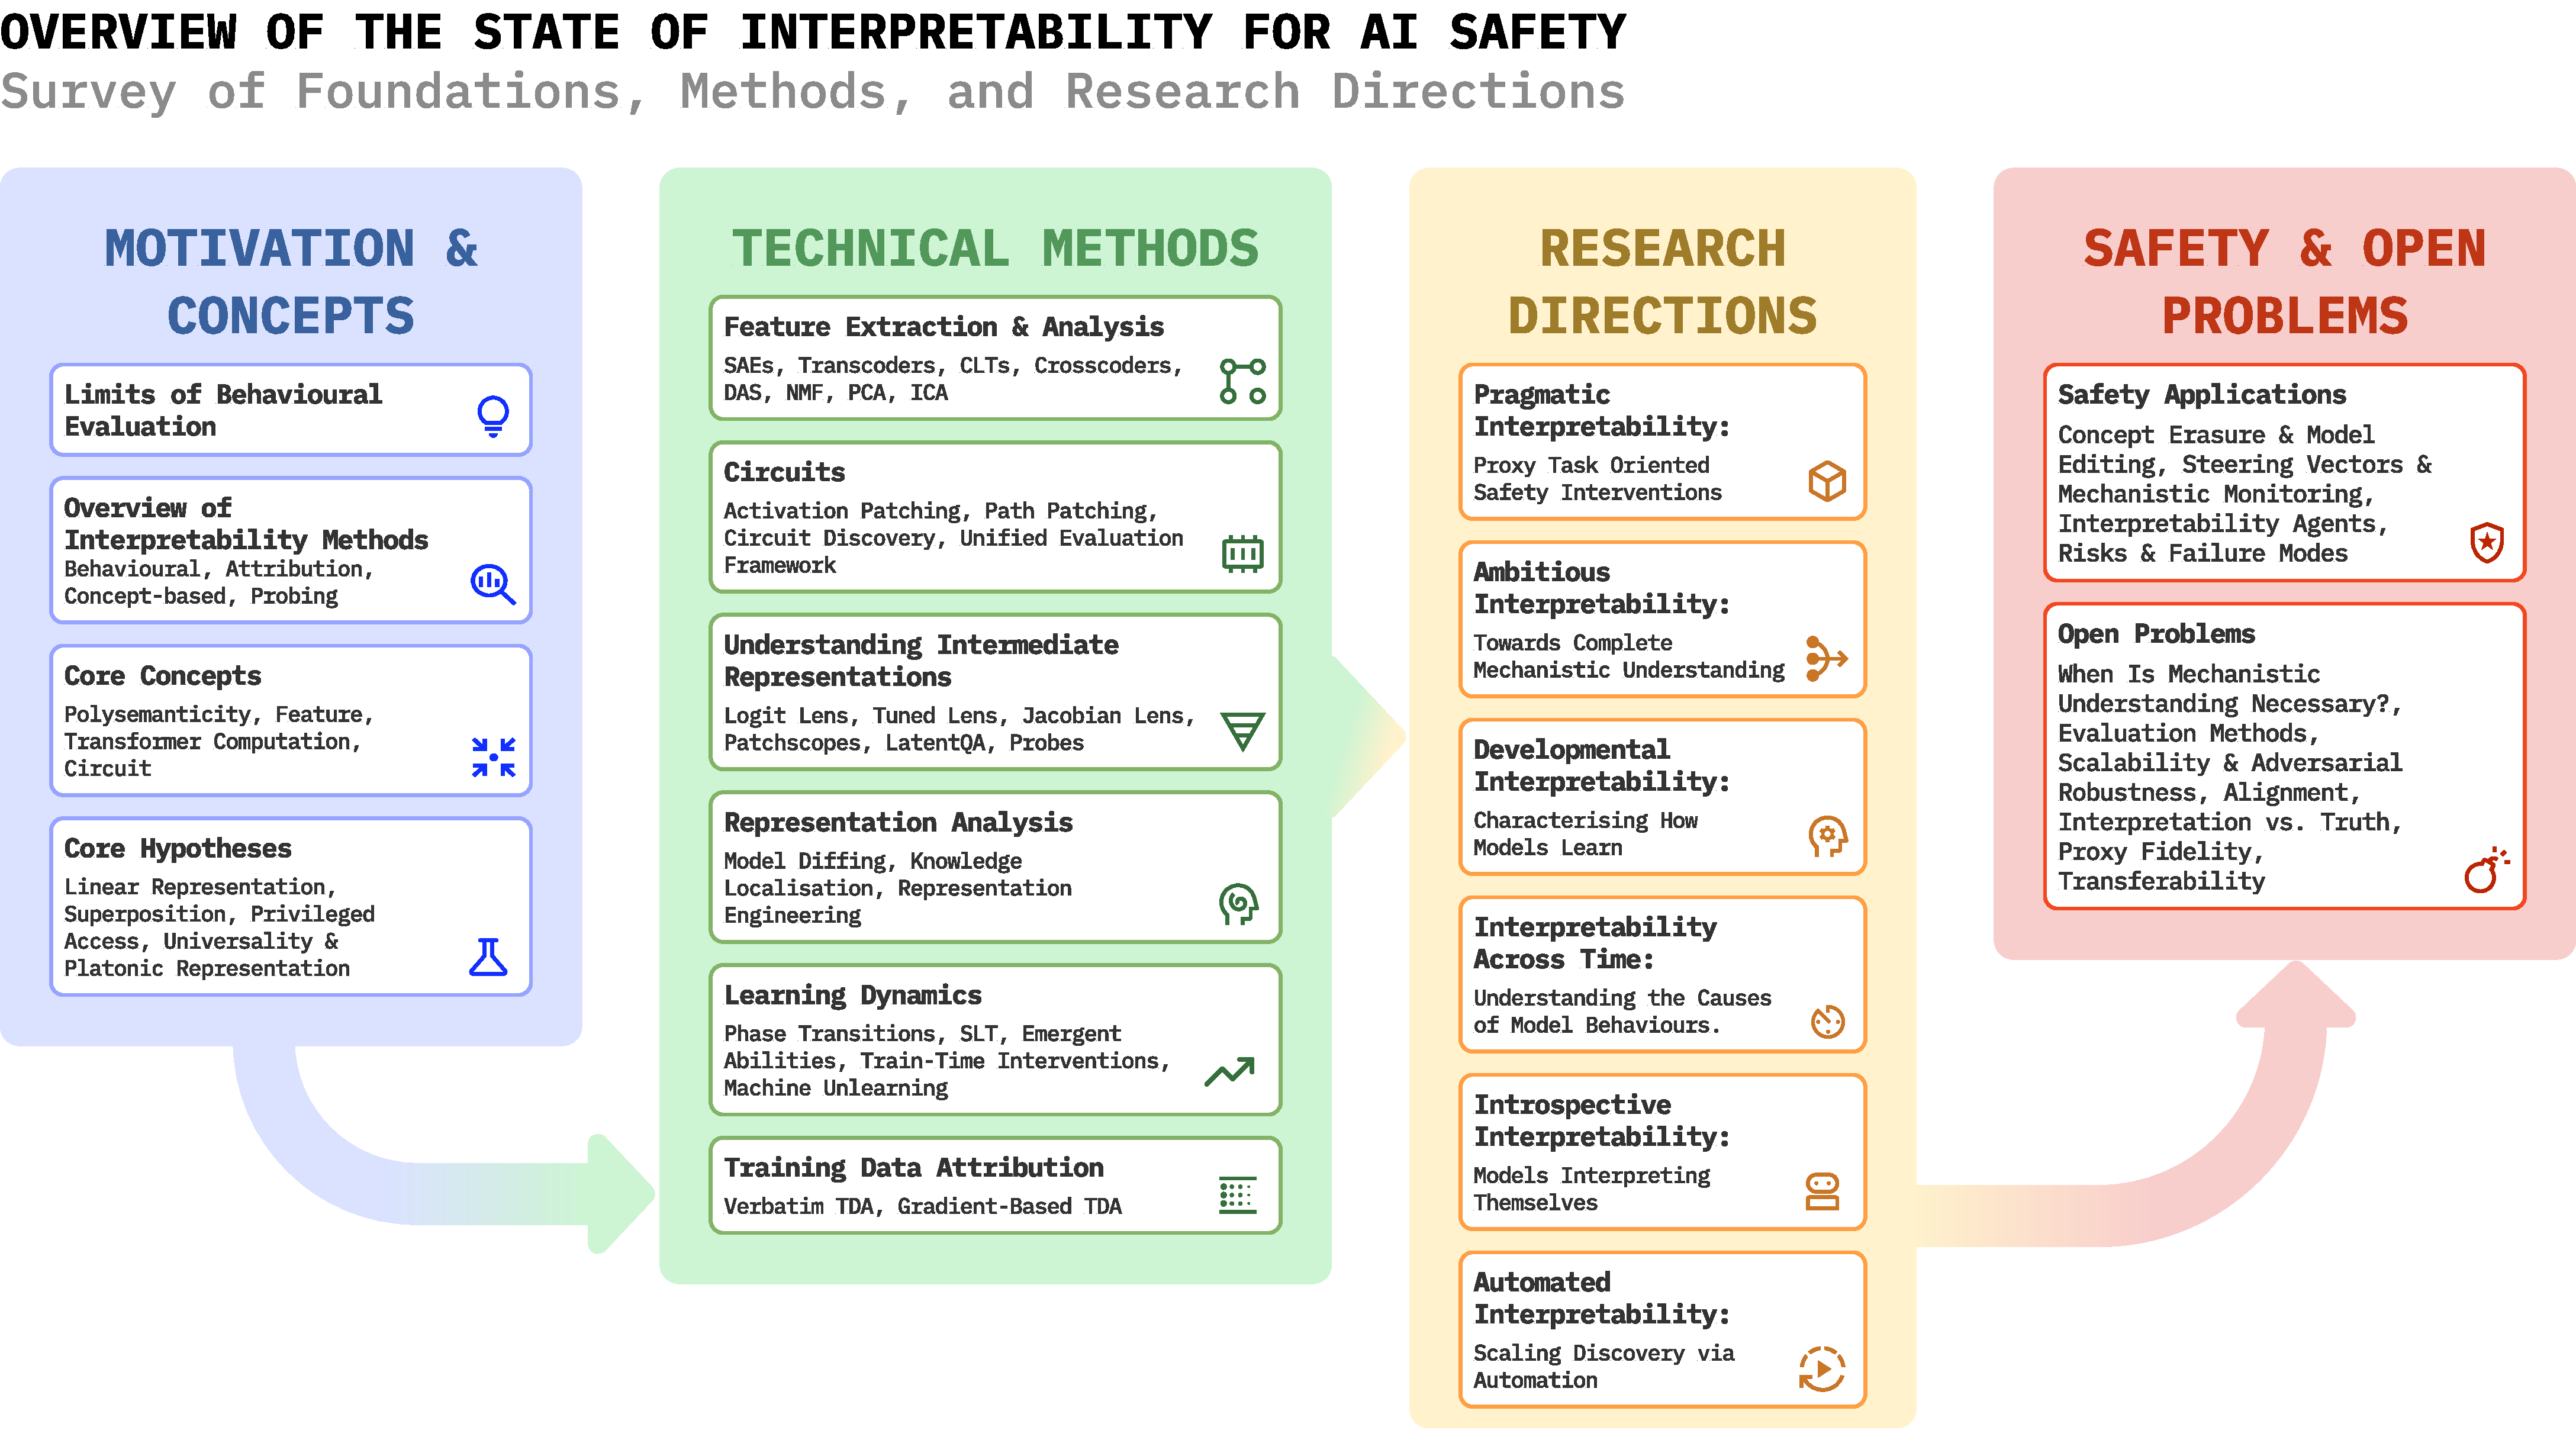
\includegraphics[width=\linewidth]{figs/1_General_summary.pdf}
  \caption{Overview of the conceptual flow of the survey, categorised into four primary pillars: (1) Motivation \& Concepts, covering fundamental knowledge and core hypotheses; (2) Technical Methods, detailing approaches developed and used in interpretability research; (3) Research Directions, exploring main directions the field is taking; and (4) Safety \& Open Problems, identifying critical challenges and deployment-oriented interventions for AI alignment.}
  \label{fig:overview}
\end{figure}



